\documentclass{style}

\begin{document}
	
	\begin{figure}
		\centering
		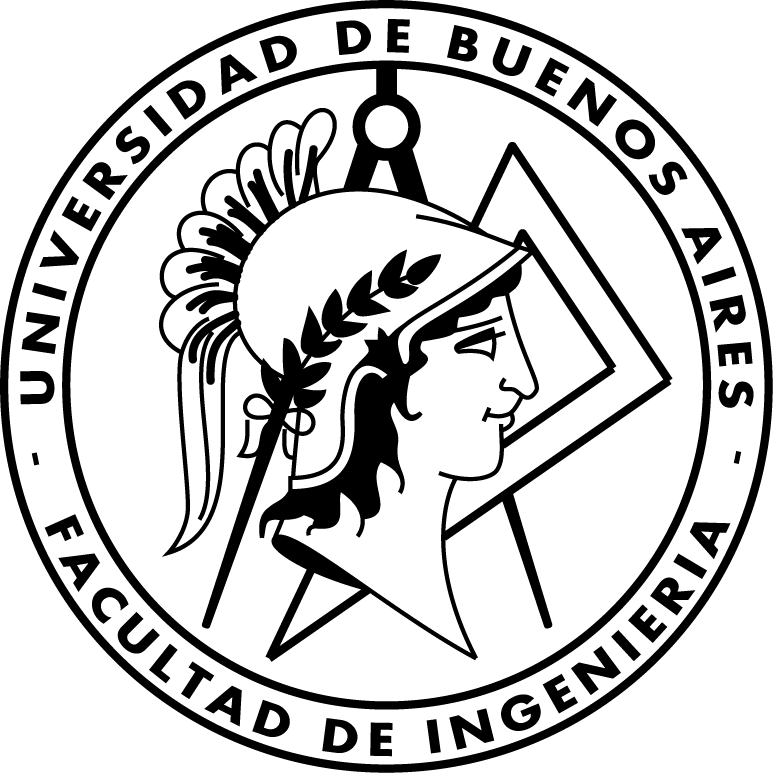
\includegraphics[scale=1.2]{logo_fiuba.png}
		\label{fig:FIUBA}
	\end{figure}
	
	\title{Análisis numérico - CB051 Modelación Numérica - Cavaliere}
	\author{Franco Secchi}
	\maketitle
    	
	\renewcommand{\contentsname}{Contenidos} 
	\begin{quote}
         \textit{Buenas buenas, esto es una guía que te dice como resolver los problemas de los finales de cavaliere. No voy a hacer tanto hincapié en las preguntas teóricas, porque las que importan son las prácticas.}
         
        \textit{Muchos éxitos en el final máquina.}
        
    \end{quote}
	\tableofcontents
    \section{Preliminares}
Vamos a dejar las formulas que mas se utilizan en los finales 

\subsection{PVI - orden = 1}
\subsubsection{Euler implicito}
$$
    y_{n+1} = y_n + h  f(y_n, t_n)
$$
¿Qué es cada cosa?

 \begin{enumerate}
     \item {$y_n$} es el valor aproximado de $y$
     \item {$y_{n+1}$} es el valor aproximado de $y$ en el siguiente paso 
     \item {$h$} es el tamaño del paso (incremento de $t$) 
     \item {$f(y_n, t_n)$} es la función que define la EDO $y' = f(y,t)$
 \end{enumerate}


\subsubsection{Ejemplos}
Dada la siguiente ecuación diferencial: 
$$y' = -y + t +1$$
Sabiendo que $y(0) = 1$

\begin{enumerate}
    \item {Calcular $u(t=1)$ con un solo avance}
    \item {Calcular $u(t=1)$ con 2 avances}
\end{enumerate} 


Para el punto 1, lo que hacemos es identificar cada termino de nuestra EDO sobre la expresión de euler implicito. 

\begin{itemize}

    \item {$f(y_n, t_n) = -y + t + 1$}
\end{itemize}

Reescribimos la formula de euler con nuestros datos. 

$$ 
y_{n+1} = y_n + h  (-y + t + 1)
$$


Para el punto 2, solamente hay que hacer 1 iteración con $t = 1$ y con $h = 1$

Calculamos $y_1$. 

$$
f(y_0, t_0) = -y_0+ t_0 + 1 = -1 + 0 + 1 = 0 
$$

Por lo tanto nos quedaría que

$$y_1 = 1 + 1*0 $$
$$y_1 = 1  $$

Entonces, con un solo avance de $h = 1$, calculamos $u(t = 1)$ y obtenemos que $u(1) = y_1 = 1$

Para el punto 2 hay que hacer lo mismo pero 2 iteraciones.
\subsubsection{Euler explicito}
$$
    y_{n+1} = y_n + h  f(y_{n + 1}, t_{n + 1})
$$
\subsubsection{Runge-Kutta de orden 2 }
$$
    q_{1u} = h  f(u_{n}, t_{n})
$$
$$
    q_{2u} = h  f(u_{n} + q_{1u}, t_{n + 1})
$$
$$
    u_{n+1} = u_n + \frac{1}{2}  (q_{1u} + q_{2u})
$$
\subsubsection{Runge-Kutta de orden 4}
\begin{align*}
q_{1_u} &= h \cdot f(u_n, t_n) \\
q_{2_u} &= h \cdot f\left(u_n + \frac{1}{2} q_{1_u}, t_n + \frac{1}{2} h\right) \\
q_{3_u} &= h \cdot f\left(u_n + \frac{1}{2} q_{2_u}, t_n + \frac{1}{2} h\right) \\
q_{4_u} &= h \cdot f\left(u_n + q3_u, t_n + h\right) \\
u_{n+1} &= u_n + \frac{1}{6} \left(q_{1_u} + 2q_{2_u} + 2q_{3_u} + q_{4_u}\right)
\end{align*}


\subsubsubsection{Observación}

Generalmente en el final te dan las formulas que vas a usar. En la gran mayoria de los casos, RK4 no lo usas ya que es eterno, a lo mejor te piden una iteración, pero no vi muchos finales que te lo pidan.

\subsection{PVI - orden mayor o igual 2 }

\begin{equation}
\left\{
\begin{array}{l}
u' = f(t,u,v) \\
v' = g(t,u,v)
\end{array}
\right.
\end{equation}

Esto queda más claro con ejercicios, tranqui que lo vamos a ver y a usar. 

\subsection{PVC}
\subsubsection{Diferencias finitas para problemas lineales}

Teniendo un problema del estilo: 


$$y'' = p(x)y' + q(x) + r(x) $$

para $a \leq x \leq b$ con $y(a) = \alpha$, $y(b) = \beta$


Al usar diferencias centradas de orden 2:

$$
y''(x_i) = \frac{y(x_{i+1}) - 2y(x_i) + y(x_{i-1}) }{h^2}
$$
$$
y'(x_i) = \frac{y(x_{i + 1}) - y(x_{i-1})}{2h}
$$

Se construye un sistema de ecuaciones lineales.

Primero vamos a hacer un cambio de variables: 

$$w_0 = \alpha, \space w_{N + 1} = \beta$$

Lo que hacemos es despejar $r(x)$, lo cual nos queda:

$$-r(x) = \frac{-w{i+1} + 2w(x_i) - w_{i-1} }{h^2} + p(x)(\frac{w_{i + 1} - w_{i - 1}}{2h}) + q(x_i)w_i $$



$$-h^2r(x) = -(1 + \frac{h}{2} p(x_i))w_{i -1} + (2 + h^2 q(x_i))w_i - (1 - \frac{h}{2} p(x_i))w_{i + 1}$$


Resulta un sistema tridiagonal $N \times N$, $Aw = b$


Ese sistema es medio un quilombo y queda asi

\begin{figure}[ht]
    \centering
    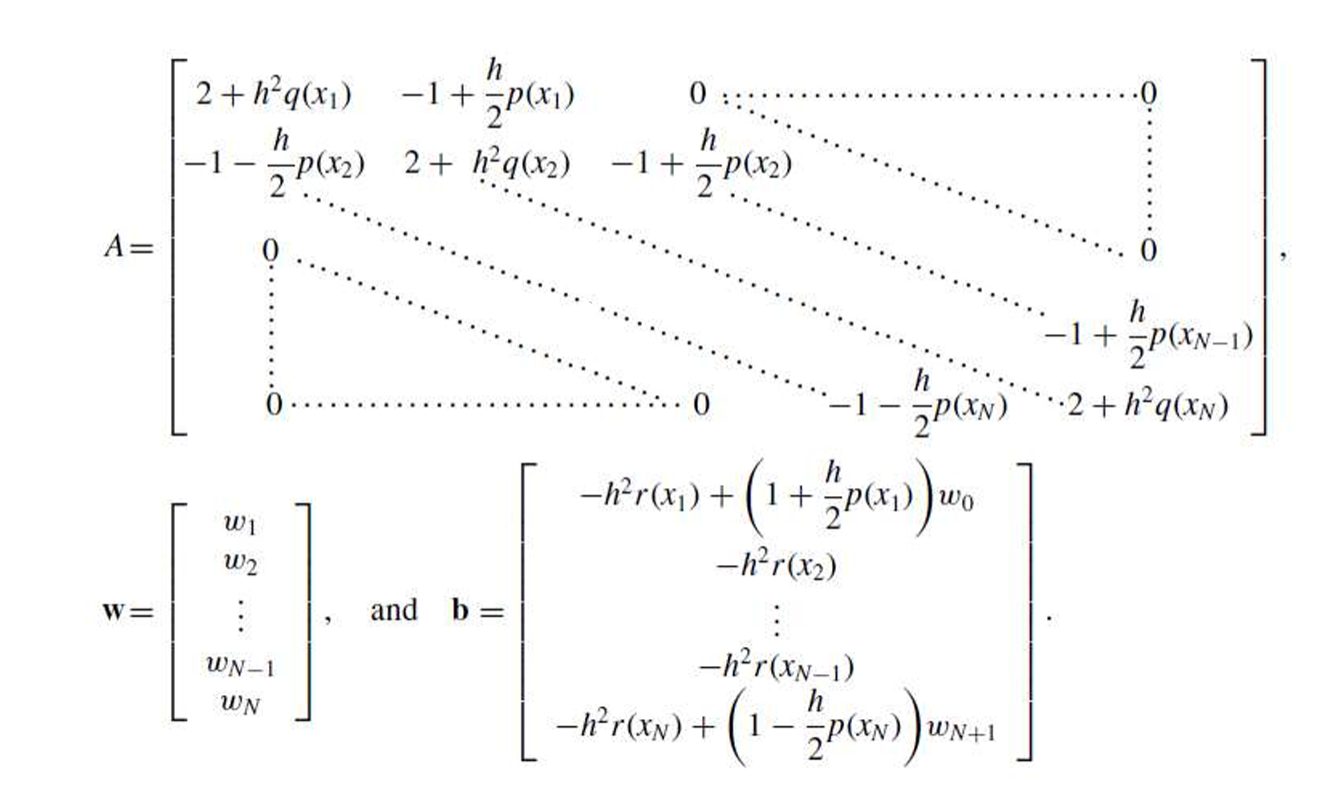
\includegraphics[width=1\linewidth]{pvc_sistema.png}
    \caption{Sistema tridiagonal}
    \label{fig:enter-label}
\end{figure}

Con los ejercicios queda mas claro, asi que chill. 


\subsection{Integración}
    \subsubsection{Trapecios}
    $$T(h) = \frac{h}{2} [f(a) + f(b) + 2\sum_{i = 1}^{N-1}f(x_{i})]$$
    
    \subsubsection{Simpson}
    $$
    S(h) = \frac{h}{3} [f(a) + f(b) + 2\sum_{k = 1}^{\frac{N-2}{2}}f(x_{2k}) + 4\sum_{k = 0}^{\frac{N-2}{2}}f(x_{2k + 1})]
    $$
    \subsubsection{Gauss}

    Tenemos la siguiente integral
    $$\int_{a}^{b} f(x) \approx \sum_{i = 0}^{n} w_if(x_i)$$

    Normalizamos de la siguiente manera: 
    $$x = \frac{(b-a)t ~+~ (b+a) }{2}$$
    $$dx = \frac{b-a}{2} dt$$

    Reemplazamos en la integral original y nos queda lo siguiente
    $$\int_{a}^{b} f(x) = \frac{b-a}{2}\int_{-1}^{1}f(\frac{(b-a)t ~+~ (b+a) }{2})dt$$
    \FloatBarrier
    \section{Problemas de valores iniciales (PVI)}

Para este tipo de ejercicios, es \textbf{siempre hacer lo mismo}. Te aprendes a como diferenciar las cosas y después es todo mecánico, lo que si tenes que ser consistente con el tema de la precisión en las cifras, aclara que vas a usar siempre 4 decimales o 5 o 7 o los que se te de la gana.

\subsection{Orden 1}

\subsubsection{02/07/2024}
La cantidad de $N$ de microbios de determinada especie evoluciona siguiendo la ley: 
$$\frac{dN}{dt} = b - aN$$

Con $a = 2$ y $b = 99$. 

En el instante inicial ($t=0$) la población de microbios es $N_0 = 98000$. Se desea determinar numéricamente la evolución de la población.

\begin{enumerate}
    \item {Discretizar mediante el siguiente método 
        \begin{equation*}
\begin{aligned}
u_{n+1} &= u_n + h f(t_n, u_n) \\
\end{aligned}
\end{equation*}
\begin{align*}
f(t_n, u_n) &= b - a u_n
\end{align*}
Adoptar para $h = 0,1$, avanzar tres pasos la solución numérica calculando $u_1, u_2, u_3$
    }

    \item { Repetir el punto anterior con el mismo valor \textbf{h} pero utilizando el siguiente método:
    \begin{equation*}
\begin{aligned}
u_{n+1} &= u_n + h/2 [f(t_{n+1}, u_{n+1}) +f(t_{n}, u_{n}) ]
\end{aligned}
\end{equation*}
\begin{align*}
f(t_n, u_n) &= b - a u_n
\end{align*}

Existe algún motivo por el cual usted pudiera indicar que este método debería proporcionar una mejor aproximación numérica. Justifique su respuesta
    }

    \item {Determinar el máximo valor de \textbf{h} a partid del cual no se puede asegurar que las perturbaciones introducidas durante el calculo no se amplifiquen durante el cálculo de la solución numérica.}
\end{enumerate}

\subsubsubsection{Resolución}

Para el punto 1, lo bueno es que ya nos dice todo, entonces solamente de ahí hay que calcular y ya esta, calculemos $u_1, u_2, u_3$

El enunciado nos dice que parte de $t = 0$ y que $N_0 = 98000$, así que al principio va a ser así: 

\begin{align*}
    u_1 &= u_0 + h(b-a*98000) \\
    u_1 &= 98000 + 0.1(99-2*98000)\\
    u_1 &= 78409.9
\end{align*}

Ahora seguimos $u_2$

\begin{align*}
    u_2 &= 78409.9 + 0.1(99-2*78409.9)\\
    u_2 &= 62737.82
\end{align*}

Por ultimo calculamos $u_3$

\begin{align*}
    u_3 &= 62737.82 + 0.1(99-2*62737.82) \\
    u_3 &= 50200.156
\end{align*}

Por lo tanto la solucion es: 
\begin{align*}
    u_1 &= 78409.9\\
    u_2 &= 62737.82\\
    u_3 &= 50200.156
\end{align*}


Vayamos al punto 2 ahora, esto es RK2, la idea es exactamente la misma, solo cambian algunas cositas. Tenemos lo siguiente:

$$ u_{n+1} = u_n + h/2 [f(t_{n+1}, u_{n+1}) +f(t_{n}, u_{n}) ] $$

Tenemos que hacer exactamente lo mismo que antes: 
\begin{align*}
    u_{1} &= u_0 + h/2 [f(t_{1}, u_{1}) +f(t_{0}, u_{0}) ]\\
    u_{1} &= 98000 + 0.1/2 [(b -au_1) + (b - a*98000)]
\end{align*}

Y lo que tenes que hacer ahí es despejar $u_1$ y así en cada iteración.

La pregunta teórica es que aunque el método RK2 y el método de Euler explícito pueden compartir una condición de estabilidad similar, como $h<2\tau h<2\tau$, RK2 sigue siendo más preciso debido a su mayor orden de convergencia.

El hecho de que RK2 sea de segundo orden significa que el error local por paso es del orden de $O(h^3)$, y el error global es del orden de $O(h^2)$. Por otro lado, el método de Euler explícito es de primer orden, con un error local por paso de O($h^2$) y un error global de $O(h)$. Esto hace que, incluso con la misma condición de estabilidad, RK2 proporcione una aproximación más precisa para un mismo tamaño de paso $h$.


Para el punto 3, lo que se hace es analizar la estabilidad. Siempre que te hablen de valor máximo o mínimo que puede tomar $h$ o algún valor de esos, es analizar estabilidad. Y se hace de la siguiente forma.

El método explícito que estás utilizando se describe como:
\[
u_{n+1} = u_n + h(b - au_n)
\]

Podemos analizar la estabilidad considerando la solución de la ecuación linealizada. La solución del método de Euler explícito es estable si:

\[
|1 - h a| < 1
\]

Este criterio asegura que las perturbaciones no se amplifican, lo que nos lleva a la siguiente condición para \( h \):

\[
-1 < 1 - h a < 1
\]

Desglosando esta desigualdad:

\[
-1 < 1 - h a \quad \text{y} \quad 1 - h a < 1
\]

\begin{enumerate}
\item De la primera parte: \( -1 < 1 - h a \)
    \[
    h a < 2 \quad \text{por lo tanto} \quad h < \frac{2}{a}
    \]
\item De la segunda parte: \( 1 - h a < 1 \)
    \[
    0 < h
    \]
\end{enumerate}

Por lo tanto, la condición final para la estabilidad es:

\[
0 < h < \frac{2}{a}
\]

Dado que \( a = 2 \), tenemos:

\[
0 < h < \frac{2}{2}
\]

\[
0 < h < 1
\]
El valor máximo de \( h \) que asegura que las perturbaciones introducidas durante el cálculo no se amplifiquen es \( 1 \). Si \( h \) es mayor a \( 1 \), el método podría volverse inestable, y las perturbaciones numéricas podrían amplificarse.

\subsubsection{12/07/2024}

Un proyectil de masa \(m = 0,11 \, \text{kg}\) que se deja caer sin velocidad inicial acelera debido a la fuerza de la gravedad y a su vez se frena por la resistencia del aire, con lo cual su ecuación de movimiento es (considerando y positivo hacia abajo)

\[
m \frac{dv}{dt} = mg - k|v|
\]

donde \(g = 9,8 \, \text{m/s}^2\) es la gravedad y \(k = 0,002 \, \text{kg/m}\) el coeficiente de resistencia del aire.

\begin{enumerate}
    \item[a)] Hallar la velocidad que alcanza el proyectil para \(t = 0,3 \, \text{s}\) utilizando el método de Euler para integrar la ecuación diferencial planteada. Sugerencia: usar un paso de cálculo de \(0,1 \, \text{s}\). (1 punto)
    \item[b)] Repetir el punto anterior utilizando el método de Runge-Kutta de orden 2. (2 puntos)
    \item[c)] Con los resultados disponibles, es posible estimar el error correspondiente al método de Euler. Justificar la respuesta. (1 punto)
\end{enumerate}

\subsubsubsection{Resolución}


Vamos a despejar la derivada para así tener nuestro $f(t,u,v)$

$$ \frac{dv}{dt} = \frac{mg - kv^2}{m}$$


Y nos pide discretizar con euler, o sea que puede ser el explicito o el implícito, podes usar el que se te de la gana. 

La idea es la misma que antes, solo que te hago la siguiente pregunta  ¿cuál es $v_0$? La rta es $v_0 = 0$, esto es porque en el enunciado nos dicen que el proyectil parte sin velocidad inicial, entonces podemos asumir que $v_0 = 0$

Tu $t_0$ es 0, ya que no te lo especifica podes asumir que si. Y vas hasta $t = 0.3$ con un paso $h = 0.1$

Para el punto $b$ que es RK2, haces lo mismo que hicimos en el ejercicio anterior (es todo bastante igual y mecánico).

Y para el punto $c$, el error de Euler en relación con RK2 se puede estimar como la diferencia entre los resultados obtenidos por ambos métodos. Si $uEuler(0.3)$ es el valor aproximado utilizando Euler y $uRK2(0.3)$ es el valor utilizando RK2, entonces el error del método de Euler se estima como:
$$\text{Error de Euler} \approx uRK2(0.3)-uEuler(0.3)$$

\subsubsection{12/12/2023}

Dado el siguiente problema de valores iniciales

\[
 \frac{dy}{dt} = \cos{y} + \frac{1}{2}t
\]


donde $y_0 = -1$.

Plantear el problema numérico con Euler explicito y calcular la solucion aproximada para t = 1, utilizando 4 pasos de tiempo. 

\subsubsubsection{Resolución}

Euler explicito es el mas simple que dice 

$$u_{n+1} = u_n + hf(t_n,u_n)$$

Es igual que los anteriores ejercicios, lo unico que no te dicen tan directo es el valor de $h$. 

Nos piden que calculemos la solucion para $t=1$ con 4 pasos de tiempo, lo que quiere decir que $h = \frac{1}{4} = 0.25$.

Y listo ahí planteas la discretización que seria: 

$$u_{n+1} = u_n + h(\cos{u_n} + \frac{1}{2} t_n)$$

Y tu $t$ parte de 0 hasta 1, con $h =0.25$.  



\subsubsection{19/07/2024}

Dado el siguiente problema de valores iniciales

\[
 \frac{dy}{dt} = 1 - y
\]


donde $y_0 = 0$.

\begin{enumerate}
    \item[a)] Determine el valor aproximado de $y$ para $t=1$ utilizando Euler explicito. Utilizando un paso de tiempo tal que haya que aplicar el método 2 veces (1 punto)
    \item[b)] Repetir el punto anterior utilizando el método de Euler implicito. (2 puntos)
    \item[c)] Analizar la estabilidad numérica de ambos métodos y calcular el paso de tiempo crítico en caso de ser necesario. Justificar la respuesta. (1 punto)
\end{enumerate}


\subsubsubsection{Resolución}

El punto A y B lo sabemos hacer, así que vamos a ir al punto C que es el que no hicimos. 


Para Euler explícito sabemos que tiene esta ecuación:

\[
y_{n+1} = y_n + h f(y_n, t_n)
\]

Sustituyendo \( f(y_n, t_n) = 1 - y_n \):

\[
y_{n+1} = y_n + h (1 - y_n)
\]

\[
y_{n+1} = y_n + h - h y_n
\]

\[
y_{n+1} = (1 - h) y_n + h
\]

El análisis de estabilidad se centra en la parte que multiplica a \( y_n \), que es \( 1 - h \). La condición de estabilidad para el método de Euler explícito es que el valor absoluto del factor de amplificación debe ser menor o igual a 1:

\[
|1 - h| \leq 1
\]

Entonces resolvemos esta desigualdad:

\[
-1 \leq 1 - h \leq 1
\]

\[
0 \leq h \leq 2
\]

Por lo tanto, el método de Euler explícito es estable para \( h \leq 2 \). El paso de tiempo crítico, \( h_{\text{crítico}} \), es 2. Si \( h > 2 \), el método se vuelve inestable.

Y para el Euler implícito tenemos su ecuación que es:

\[
y_{n+1} = y_n + h f(y_{n+1}, t_{n+1})
\]

Sustituyendo \( f(y_{n+1}, t_{n+1}) = 1 - y_{n+1} \):

\[
y_{n+1} = y_n + h (1 - y_{n+1})
\]

\[
y_{n+1} = y_n + h - h y_{n+1}
\]

\[
y_{n+1} + h y_{n+1} = y_n + h
\]

\[
y_{n+1} (1 + h) = y_n + h
\]

\[
y_{n+1} = \frac{y_n + h}{1 + h}
\]

Para el método de Euler implícito, el factor de amplificación es:

\[
\frac{1}{1 + h}
\]

El método es estable si el valor absoluto del factor de amplificación es menor o igual a 1:

\[
\left|\frac{1}{1 + h}\right| \leq 1
\]

Esta condición es \textbf{siempre cierta} para cualquier \( h \geq 0 \), lo que significa que el método de Euler implícito es incondicionalmente estable. No hay un paso de tiempo crítico que deba calcularse, ya que el método es estable para cualquier \( h \).




\subsection{Orden mayor o igual a 2}

No hay muchos finales con este tipo de ejercicios. Hago un par que encontré. La lógica es \textbf{siempre} la misma.

\subsubsection{30/07/24}
Dado el siguiente problema de valores iniciales

$$
    \frac{d^2y}{dt^2} = t^2
$$
Con $y_0 = 0$ y $\frac{dy}{dt}_0 = 1$

\begin{enumerate}
    \item[a)] Discretizar por el método de Euler Explicito y dejar planteado el problema numérico resultante para un paso de tiempo $k$ genérico (1 punto)
    \item[b)] Tomar $k = 0.1$ y obtener una aproximación de y en $t=0.3$ (usando el problema numérico definido en el punto anterior) (2 puntos)
    \item[c)] Discretizar por el método de Euler implicito. Calcular para un solo paso de tiempo con $k=0.1$ (1 punto)
\end{enumerate}

\subsubsubsection{Resolución}

Para hacer el punto (a) recordemos lo que habíamos dicho en las preliminares: 

\begin{equation}
\left\{
\begin{array}{l}
u' = f(t,u,v) \\
v' = g(t,u,v)
\end{array}
\right.
\end{equation}


Lo que hacemos es hacer un cambio de variables. Vamos a decir lo siguiente 
$$v(t) = \frac{dy}{dt'}$$
$$u(t) = y(t)$$

Entonces si nosotros derivamos $u(t)$, tenemos a $v(t)$ y si derivamos $v(t)$, estaría representando a $y''$. Por lo tanto tendríamos lo siguiente:

\begin{equation}
\left\{
\begin{array}{l}
u' = v(t) \\
v' = y'' = t^2
\end{array}
\right.
\end{equation}

En estos casos, hay que discretizar las \textbf{dos} ecuaciónes. Y nos quedaria así 

\begin{equation}
\left\{
\begin{array}{l}
u_{n+1} = u_n + kv_n(t) \\
v_{n+1} = v_n + kt_n^2
\end{array}
\right.
\end{equation}

Y este es el problema numérico resultante para un paso de tiempo k genérico.

Para el punto (b) solo queda resolver. Vamos a calcular los valores de \( u \) y \( v \) para \( t = 0.1 \), \( t = 0.2 \), y \( t = 0.3 \), usando \( k = 0.1 \).

\begin{itemize}
    \item Para \( t = 0.1 \):
    \[
    u_1 = u_0 + k v_0 = 0 + 0.1 \times 1 = 0.1
    \]
    \[
    v_1 = v_0 + k t_0^2 = 1 + 0.1 \times 0^2 = 1
    \]
    
    \item Para \( t = 0.2 \):
    \[
    u_2 = u_1 + k v_1 = 0.1 + 0.1 \times 1 = 0.2
    \]
    \[
    v_2 = v_1 + k t_1^2 = 1 + 0.1 \times 0.1^2 = 1 + 0.001 = 1.001
    \]
    
    \item Para \( t = 0.3 \):
    \[
    u_3 = u_2 + k v_2 = 0.2 + 0.1 \times 1.001 = 0.2 + 0.1001 = 0.3001
    \]
    \[
    v_3 = v_2 + k t_2^2 = 1.001 + 0.1 \times 0.2^2 = 1.001 + 0.004 = 1.005
    \]
\end{itemize}

Por lo tanto, la aproximación de \( y \) (que es \( u \)) en \( t = 0.3 \) es \( y(0.3) \approx 0.3001 \).

Y ahora resolvamos el punto C. 
Aplicando el método de Euler implícito, las ecuaciónes son:

\begin{equation}
\left\{
\begin{array}{l}
u_{n+1} = u_n + k v_{n+1} \\
v_{n+1} = v_n + k t_{n+1}^2
\end{array}
\right.
\end{equation}

Con \( k = 0.1 \), vamos a calcular \( u_1 \) y \( v_1 \):

Primero vamos a tener que calcular $v_1$, ya que lo necesitamos para calcular $u_1$.

\[
v_1 = v_0 + k t_1^2 = 1 + 0.1 \times 0.1^2 = 1.001
\]
\[
u_1 = u_0 + k v_1 = 0 + 0.1 \times 1.001 = 0.1001
\]

Por lo tanto, para un solo paso de tiempo con \( k = 0.1 \), tenemos:

\[
u_1 \approx 0.1001, \quad v_1 \approx 1.001
\]
\subsubsection{18/12/13}

Considere el siguiente oscilador armónico: 

$$
    \frac{d^2\theta}{dt^2} + \frac{g}{L}\theta = 0
$$

Con $g=9.8 \frac{m}{s^2}$, $L = 0.49m$, $\theta_0 = \frac{\pi}{20}$ y $\frac{d\theta}{dt}_0 = 0$


\begin{enumerate}
    \item[a)] Discretizar por el método de Euler Explicito 
\end{enumerate}


\subsubsubsection{Resolución}

Se plantea el mismo cambio de variables del anterior ejercicio: 

\begin{equation}
\left\{
\begin{array}{l}
\theta' = v(t) \\
v' = \theta'' = -\frac{g}{L}\theta
\end{array}
\right.
\end{equation}


Entonces con esta info, discretizamos: 
\begin{equation}
\left\{
\begin{array}{l}
\theta_{n+1} = \theta_n + k v_{n+1} \\
v_{n+1} = v_n + k (-\frac{g}{L}\theta_n)
\end{array}
\right.
\end{equation}

Y listo. Si te piden para un tiempo especifico, empezas a reemplazar los valores e iteras.




    \FloatBarrier
    \section{Problemas de valores de contorno (PVC)}
Para este tipo de ejercicios también, es \textbf{siempre hacer lo mismo}. Te aprendes a como armar la matriz y las 2 formulas (tal vez 3) de diferenciación y después es todo mecánico. Vas a ver que te van a pedir utilizar metodos vistos en clase para resolver sistemas de ecuaciones. Anda a la fácil, usa Gauss-Seidel o Jacobi (ahre que son las unicas. Porque SOR no vas a usarlo, querete un poco).


\subsection{6/08/24}

Sea la ecuación diferencial

$$\frac{d^2y}{dx^2} + \frac{y}{4} = 0$$

con $y_0 = 1$ y $y_\pi = 0$

Plantear su resolución numerica usando diferencias finitas centradas. Expresar el sistema de ecuaciones resultantes en forma matricial. Considerar que el dominio se divide en $N + 1$ tramos.

\begin{enumerate}
    \item[a)] Obtener la solución aproximada para $N = 1$ (1 punto)
    \item[b)] Repetir para $N = 3$. Usar métodos vistos en el curso para resolver sistema lineal(2 puntos)
    \item[c)]Estimar el valor de $y(\frac{\pi}{2})$(1 punto)
\end{enumerate}

\subsubsection{Punto a}

Que nos digan que el dominio esta dividido en $N + 1$ tramos nos dice que va a haber $N$ puntos sin contar los bordes.


Discretizamos. Para esto utilizamos las formulas de las preliminares. 


$$
y''(x_i) = \frac{y(x_{i+1}) - 2y(x_i) + y(x_{i-1}) }{h^2}
$$

Ahora lo que hacemos es reemplazamos en la ecuación diferencial original. 



$$
\frac{y(x_{i+1}) - 2y(x_i) + y(x_{i-1}) }{h^2} + \frac{y_n}{4} = 0
$$


Multiplicamos $h^2$ en ambos miembros, agrupamos y reorganizamos. 


$$
    \textcolor{green}{(1)}y_{n+1} + \textcolor{blue}{(-2 + \frac{h^2}{4})}y_n + \textcolor{red}{(1)}y_{n-1} = 0  
$$

Bien, acá remarcamos los coeficientes que multiplican a las $y$ porque son los que van a ir a las matrices. 

Así que con esto, podemos armar la matriz generica. Recordemos como queda la parte después del igual de la matriz: 
\newpage
\begin{figure}[h!]
    \centering
    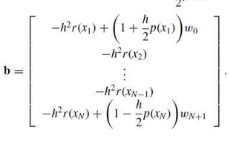
\includegraphics[width=0.5\linewidth]{b_matrix_pvc.png}
    \caption{Sistema tridiagonal}
    \label{fig:enter-label}
\end{figure}

Como podes observar, en el primer elemento esta el $-h^2 r(x_1)$, Que es lo que queda a la derecha del igual de la ecuación diferencial ya despejada y ya discretizada. Y después tiene un $(\dots)w_0$, ese $w_0$ es el dato que te dan de $y_0$. Para la primera iteración pasas el $y_{n-1}$ para el otro lado del igual, y el valor que lo acompaña es su coeficiente. La matriz es \textbf{siempre igual}.

Sabiendo esto, vamos a armar la matriz: 

\[
\begin{bmatrix}
\textcolor{blue}{(-2 + \frac{h^2}{4})} & \textcolor{green}{(1)} & 0 & \dots & 0 \\
\textcolor{red}{(1)} & \textcolor{blue}{(-2 + \frac{h^2}{4})} & \textcolor{green}{(1)} & \dots & 0 \\
\dots  & \dots  & \dots  & \dots & \dots  \\
0 & 0 & \dots & \textcolor{green}{(1)} & \textcolor{blue}{(-2 + \frac{h^2}{4})}
\end{bmatrix}
\begin{bmatrix}
y_1 \\ y_2 \\ \dots \\ y_n 
\end{bmatrix}
=
\begin{bmatrix}
-y_0 \\ 0 \\ \dots \\ -y_{n+1}
\end{bmatrix}
\]

Y esta es la matriz genérica. 

\subsubsection*{Calculamos la solución para $N=1$}

¿Cuál es el valor de $h$? Bueno, para calcularlo se hace lo siguiente: 

$$h = \frac{L_s - L_i}{N+1}$$

Siendo $L_s$ el limite superior y $L_i$ el inferior. Esto lo sacas de los valores que te dan, por ejemplo te dan los datos para $y_0$ y para $y_{\pi}$, entonces tu rango es $[0, \pi]$

$$h = \frac{\pi - 0}{1+1} = \frac{\pi}{2}$$

Como me piden la solución para $N=1$, eso nos dice que solamente va a haber un punto sin contar el borde, que es $x_1 = \frac{\pi}{2}$.

La matriz que generamos es de $N\times N$, solamente nos va a queda una ecuación.


$$y_2 + (-2 + \frac{h^2}{4})y_1 = -1$$

$y_2 = 0$, esto es porque $y_{\pi} = 0 $.

$$0 + (-2 + \frac{(\frac{\pi}{2})^2}{4})y_1 = -1$$


Despejamos $y_1$

$$y_1 \approx 0.722987 $$


\subsubsection{Punto b}

Nos dicen que $N = 3$, entonces nuestro $h$ va a cambiar, la cantidad de puntos también, que van a ser tres puntos, y la dimensión de la matriz va a ser de $3\times 3$. 

Calculamos nuestra nueva $h$: 
$$h = \frac{\pi}{ 3+ 1} = \frac{\pi}{4}$$

Y analizamos cuales van a ser nuestros puntos: $x_1=\frac{\pi}{4}$, $x_2 = \frac{\pi}{2}$, $x_3 = \frac{3\pi}{4}$

La matriz que nos habia quedado era la siguiente

\[
\begin{bmatrix}
\textcolor{blue}{(-2 + \frac{h^2}{4})} & \textcolor{green}{(1)} & 0 & \dots & 0 \\
\textcolor{red}{(1)} & \textcolor{blue}{(-2 + \frac{h^2}{4})} & \textcolor{green}{(1)} & \dots & 0 \\
\dots  & \dots  & \dots  & \dots & \dots  \\
0 & 0 & \dots & \textcolor{green}{(1)} & \textcolor{blue}{(-2 + \frac{h^2}{4})}
\end{bmatrix}
\begin{bmatrix}
y_1 \\ y_2 \\ \dots \\ y_n 
\end{bmatrix}
=
\begin{bmatrix}
-y_0 \\ 0 \\ \dots \\ -y_{n+1}
\end{bmatrix}
\]

Reemplazamos los nuevos valores y nos quedaria lo siguiente

\[
\begin{bmatrix}
\textcolor{blue}{-1,845787} & \textcolor{green}{(1)} & 0 \\
\textcolor{red}{(1)} & \textcolor{blue}{-1,845787} & \textcolor{green}{(1)}  \\
0 & \textcolor{green}{(1)} & \textcolor{blue}{-1,845787}
\end{bmatrix}
\begin{bmatrix}
y_1 \\ y_2 \\ y_3 
\end{bmatrix}
=
\begin{bmatrix}
-1 \\ 0 \\ 0
\end{bmatrix}
\]


Y nos piden usar algun método utilizado en clase, por ejemplo usemos Gauss-Seidel. 



\begin{equation}
\left\{
\begin{array}{l}
y^{k+1}_1 = \frac{-1 - y^k_2}{-1,845787} \\ \\
y^{k+1}_2 = \frac{-y^k_3 - y^{k+1}_1}{-1,845787} \\ \\
y^{k+1}_3 = \frac{ - y^{k+1}_2}{-1,845787} 
\end{array}
\right.
\end{equation}


Y vos te estarás preguntando ¿Cual es la semilla? ¿Cuantas iteraciones tengo que hacer? ¿Lo hago teniendo en cuenta el error? 

Bueno, la semilla puede ser la que vos quieras, anda con la semilla más fácil que es  $y = [0,0,0]^T$. Y con respecto a las otras dos preguntas, podes tomar dos caminos para resolver el problema: 

\begin{enumerate}
    \item {Realizas $n$ iteraciones (las que vos quieras, que en realidad son las que puedan parecer \textit{más} coherentes)}
    \item {Iterar hasta que supere cierto error (que es el que vos quieras, por ejemplo $\Delta y \leq 0.001$)}
\end{enumerate}

La más fácil es la primera y la \textit{más correcta} es la segunda (yo fui por la primera y no hubo drama).

Haces la solución que quieras y listorti. 


\subsubsection{Punto C}

Como nuestra matriz era de $3 \times 3 $, y nuestro punto $x_2 = \frac{\pi}{2}$, el último valor que hayamos sacado para $y_2$ en nuestro sistema de ecuaciones, es la solución. 

\subsection{02/07/24}

Sea la ecuación diferencial

$$\frac{d^2y}{dx^2} = -a\frac{dy}{dx}$$

con $0 \leq x \leq 1$ y unas condiciones de contorno de $y_0 = 0$ y $y_1 = 1$

Plantear su resolución numerica usando diferencias finitas centradas. Expresar el sistema de ecuaciones resultantes en forma matricial. Considerar que el dominio se divide en $N + 1$ tramos.

\begin{enumerate}
    \item[a)] Obtener la solución aproximada para $a = 1$ y $N = 1$ (1 punto)
    \item[b)] Repetir para $N = 3$. Usar métodos vistos en el curso para resolver sistema lineal(2 puntos)
    \item[c)] Existe en este caso alguna limitación para el tamaño del paso espacial $\delta x$. De ser así encontrar el tamaño de paso espacial máximo para $a = 1$ (1 punto)
\end{enumerate}

\subsubsection{Punto C}

Para analizar la estabilidad del método de diferencias finitas centradas aplicado a la ecuación diferencial:

\[
\frac{d^2y}{dx^2} = -a\frac{dy}{dx}
\]

con las condiciones de contorno \( y(0) = 0 \) y \( y(1) = 1 \), y considerando que el dominio se divide en \( N + 1 \) tramos, procedemos de la siguiente manera:

Usamos diferencias finitas centradas para aproximar las derivadas:

\[
\frac{d^2y}{dx^2} \approx \frac{y_{i-1} - 2y_i + y_{i+1}}{h^2}
\]
\[
\frac{dy}{dx} \approx \frac{y_{i+1} - y_{i-1}}{2h}
\]

Sustituyendo estas aproximaciones en la ecuación diferencial, obtenemos:

\[
\frac{y_{i-1} - 2y_i + y_{i+1}}{h^2} = -a\frac{y_{i+1} - y_{i-1}}{2h}
\]

Multiplicando por \( h^2 \):

\[
y_{i-1} - 2y_i + y_{i+1} = -a \frac{h}{2} (y_{i+1} - y_{i-1})
\]

Reordenando la ecuación:

\[
y_{i-1} \left(1 + \frac{ah}{2}\right) - 2y_i + y_{i+1} \left(1 - \frac{ah}{2}\right) = 0
\]

Para que el método sea estable, consideramos la condición:

\[
|1 - \frac{a h}{2}| \leq 1
\]

Resolviendo esta desigualdad:

\[
1 - \frac{ah}{2} \leq 1 \quad \text{y} \quad 1 - \frac{a h}{2} \geq -1
\]

La primera parte es siempre cierta. La segunda parte da:

\[
-\frac{a h}{2} \geq -2
\]

Simplificando:

\[
h \leq \frac{2}{a}
\]

Por lo tanto, la condición de estabilidad es:

\[
a h \leq 2
\]

Para \( a = 1 \), la condición de estabilidad se convierte en:

\[
h \leq 2
\]

Esto significa que el tamaño máximo del paso espacial permitido es \( h = 2 \).




\subsection{30/07/24}

Sea la ecuación diferencial

$$-2\frac{d^2y}{dx^2} + y = e^{-0.2x}$$

con $y_0 = 1$ y $y_2 = 1$

Plantear su resolución numerica usando diferencias finitas centradas. Expresar el sistema de ecuaciones resultantes en forma matricial. Considerar que el dominio se divide en $N + 1$ tramos.

\begin{enumerate}
    \item[a)] Obtener la solución aproximada para $N = 1$ (1 punto)
    \item[b)] Repetir para $N = 3$. Usar métodos vistos en el curso para resolver sistema lineal(2 puntos)
    \item[c)] Si la condicion de borde en $x = 2$ fuera $\frac{dy}{dx} = 0$ explicar que cambios habría que efectuar en el planteo de la resolución numérica del problema.(1 punto)
\end{enumerate}

\subsubsection{Observaciones}

En este ejercicio hay un dato que hasta el momento no usamos, que es $x$. ¿Cómo hago si tengo una $x$ ahí? El valor de $x$ va a ir cambiando con las iteraciones, y se calcula de la siguiente manera: 
$$x_i = L_i + ih$$

Siendo $L_i$ el limite inferior, $i \in N\ $ y el $h$ el de toda la vida.


\subsubsection{Punto a}

Discretizamos la ecuación diferencial

$$
-2\frac{y_{i-1} - 2y_i + y_{i+1}}{h^2} + y_n = e^{-0.2x_i} 
$$

Distribuimos y reorganizamos

$$
\textcolor{green}{(\frac{-2}{h^2})}y_{i+1} + \textcolor{blue}{(\frac{4}{h^2} + 1)}y_i + \textcolor{red}{(\frac{-2}{h^2})}y_{i-1} = e^{-0.2x_i} 
$$

Con esto armamos la matriz: 


\[
\begin{bmatrix}
\textcolor{blue}{(\frac{4}{h^2} + 1)} & \textcolor{green}{(\frac{-2}{h^2})} & 0 & \dots & 0 \\
\textcolor{red}{(\frac{-2}{h^2})} & \textcolor{blue}{(\frac{4}{h^2} + 1)}  & \textcolor{green}{(\frac{-2}{h^2})} & \dots & 0 \\
\dots  & \dots  & \dots  & \dots & \dots  \\
0 & 0 & \dots & \textcolor{green}{(\frac{-2}{h^2})}  & \textcolor{blue}{(\frac{4}{h^2} + 1)}
\end{bmatrix}
\begin{bmatrix}
y_1 \\ y_2 \\ \dots \\ y_n 
\end{bmatrix}
=
\begin{bmatrix}
e^{-0.2x_i}  + \textcolor{red}{(\frac{2}{h^2})}y_0  \\ e^{-0.2x_i}  \\ \dots \\  e^{-0.2x_i}  +\textcolor{green}{(\frac{2}{h^2})}y_{n+1}
\end{bmatrix}
\]



\subsubsection*{Resolvemos para $N = 1$}

Calculamos $h$

$$h = \frac{2 - 0}{ 1 + 1} = \frac{2}{2} = 1$$

Ahora planteamos la ecuación y despejamos $y_1$

$$
(\frac{-2}{h^2})y_2 + (\frac{4}{h^2} + 1)y_1 = e^{-0.2(0 + 1*1)} + (\frac{2}{h^2})y_0
$$

$$
-2 * 0 + 5y_1 = e^{-0.2(0 + 1*1)} + 2 * 1
$$


$$
y_1 \approx 0.5637
$$


\subsubsection{Punto c}

Si esa es la nueva condición, nuestro problema se convierte en uno con una frontera del tipo Neumman en lugar de Dirichlet. Con esta condición se implementa lo siguiente: 

$$
    y' \approx \frac{y_{n +1} - y_{n- 1}}{2h}
$$


Como $y'_2 = 0$ 

$$
    0 = \frac{y_{n +1} - y_{n- 1}}{2h}
$$

Multiplicamos $2h$ y despejamos

$$
     y_{n +1} = y_{n- 1}
$$

Con dicha igualdad, tenemos que ajustar en nuestra matriz la ultima fila, indicando que

$$ y_{n +1} = y_{n- 1} $$

Por lo tanto la ultima fila quedaría de la siguiente manera: 

$$  e^{-0.2x_i}  +(\frac{2}{h^2})y_{n-1}$$

\subsection{12/12/23}

Sea la ecuación diferencial

$$\frac{d^2y}{dx^2} + 3x = 2$$

con $y_0 = 1$ y $y_1 = 0$

\begin{enumerate}
    \item[a)] Se pide Plantear su resolución numérica usando diferencias finitas centradas. Expresar el sistema de ecuaciones resultantes en forma matricial. Considerar que el dominio se divide en $N + 1$ tramos. (1 punto)
    \item[b)] Resolver para $N = 2$. (2 puntos)
    \item[c)] Utilizando los resultados de b) y los datos del problema, obtener un polinomio que interpole la solución aproximada utilizado alguno de los métodos vistos en el curso.
\end{enumerate}

\subsubsection{Punto c}

Este ejercicio esta piola porque te mezcló varios temas. Supongamos que en el punto b te da que $y_1 = \frac{13}{27} $ $ y_2 = \frac{5}{27} $, y te piden un polinomio que interpole... acá podes usar interpolacion de Newton o de Lagrange, la que se te sea más cómoda. Yo usé la de Newton.


Entonces tenemos esta tablita de valores 

\begin{center}
\begin{tabular}{ | m{1em} | m{1cm} | m{1cm} | m{1cm} | m{1cm} | } 
  \hline
  i & 0 & 1 & 2 & 3 \\ 
  \hline
  x & 0 & $\frac{1}{3}$ & $\frac{2}{3}$ & 1 \\ 
  \hline
  y & 1 & $\frac{13}{27}$ & $\frac{5}{27}$ & 0 \\ 
  \hline
\end{tabular}
\end{center}


Y con esto vamos a plantear la interpolación de Newton.

\[
\begin{array}{c | c | c | c | c}
\toprule
x & y & \text{Primeras diferencias divididas} & \text{SDD} & \text{TDD } \\
\midrule
x_0 = 0 & 1 & \textcolor{red}{f[x_1, x_0] = \frac{\frac{13}{27} - 1}{\frac{1}{3} - 0} = \frac{-14}{9}} & 1 & \frac{-1}{2}\\
\midrule
x_{1} = \frac{1}{3} & \frac{13}{27} & \textcolor{red}{f[x_2, x_1] = \frac{-8}{9}} & \frac{1}{2} & \\
\midrule
x_{2} = \frac{2}{3} & \frac{5}{27} & \textcolor{red}{f[x_3, x_2] = \frac{-5}{9}} &  \\
\midrule
x_3 = 1 & 0 & & & \\
\bottomrule
\end{array}
\]

El polinomio de interpolación de Newton es:

\[
p(x) = 1 + \left(\frac{-14}{9}\right) \cdot x + \left(1\right) \cdot x(x - \frac{1}{3}) + \left(\frac{-1}{2}\right) \cdot x(x - \frac{1}{3})(x - \frac{2}{3})
\]


Simplificando nos quedaría que: 
\[
p(x) = \frac{8}{9} - \frac{2}{9}x + \frac{1}{2}x^2
\]

    \FloatBarrier
    \section{Integración}

\subsection{16/07/24}

Conociendo los valores de $f(x)$ presentados en la siguiente tabla

\begin{center}
\begin{tabular}{ |c|c|c|c|c|c|c|c|c|c| } 
 \hline
 $x$ & $3.4$ & $3.6$ & $3.8$ & $4.0$& $4.2$ & $4.4$ & $4.6$ & $4.8$ & $5.0$ \\ 
 \hline
 $f(x)$ & $12.426$ & $12.208$ & $11.984$ & $11.573$ & $11.399$ & $11.270$ & $11.190$ & $11.254$ & $11.304$ \\ 
 \hline
\end{tabular}
\end{center}



\begin{enumerate}
    \item[a)]Utiliza la regla del Trapecio para aproximar el valor de la integral de la función $f(x)$ sobre el intervalo $[3.4 ; 5.0]$ tomando $h = 0.2$ (1 punto)
    \item[b)] Repetir el caso anterior con $h = 0.4$ y utilizar estos dos resultados del método para obtener una mejor aproximación de la integral solicitada. Justificar respuesta. (2 puntos)
    \item[c)] ¿Es posible obtener una estimación de la integral buscada mejor que todas las aproximaciones obtenidas anteriormente?. Explicar cómo justificando la respuesta (1 punto)
\end{enumerate}


\subsubsection{Punto a}

\[
T(h) \approx \frac{0.2}{2} \left[ 12.426 + 2 \left(12.208 + 11.984 + 11.573 + 11.399 + 11.270 + 11.190 + 11.254 \right) + 11.304 \right]
\]

\[
I \approx 0.1 \cdot 185.086 = 18.5086
\]

 \subsubsection{Punto b}
 
Utilizando la regla del Trapecio con \( h = 0.4 \):

\[
T(h) \approx \frac{0.4}{2} \left[ 12.426 + 2 \left(11.984 + 11.399 + 11.190 \right) + 11.304 \right]
\]

\[
T(h) \approx 0.2 \cdot 93.832 = 18.5752
\]

Usando la extrapolación de Richardson para obtener una mejor aproximación:

$$
I_{\text{mejor}} = \frac{4I_{h/2} - I_{h}}{3}
$$

\[
I_{\text{mejor}} = \frac{4 \cdot 18.5752 -  18.5086}{3} = 18.5974
\]

\subsubsection{Punto c}
Para obtener una estimación mejor que las obtenidas anteriormente, se puede utilizar un valor de \( h \) más pequeño utilizar la extrapolación de Richardson, ya que es una técnica que mejora la precisión combinando resultados de diferentes valores de \( h \).


\end{document}
